\subsection{Gestion des stocks intelligente}

La gestion des stocks au sein d'une entreprise doit permettre de ne jamais manquer de quoi que ce soit, tout en faisant attention à ne pas trop acheter dans le souci d'économiser de l'argent.
Il faut constamment anticiper les besoins afin d'acheter au bon moment, ce qui n'est pas chose facile.
Dans cette section nous allons voir comment l'intelligence artificielle peut aider à simplifier la gestion des stocks des entreprises.

Dans de grandes compagnies qui doivent gérer des stocks immenses, il y a de plus en plus d'automatisation.
Par exemple, \textsc{Amazon} a automatisé, grâce à l'intelligence artificielle et des robots, la plupart des fonctions d'enlèvement/ramassage, d'emballage et de stockage.

\FloatBarrier
\begin{figure}[h!]
    \begin{minipage}[c]{0.55\textwidth}
        \begin{center}
            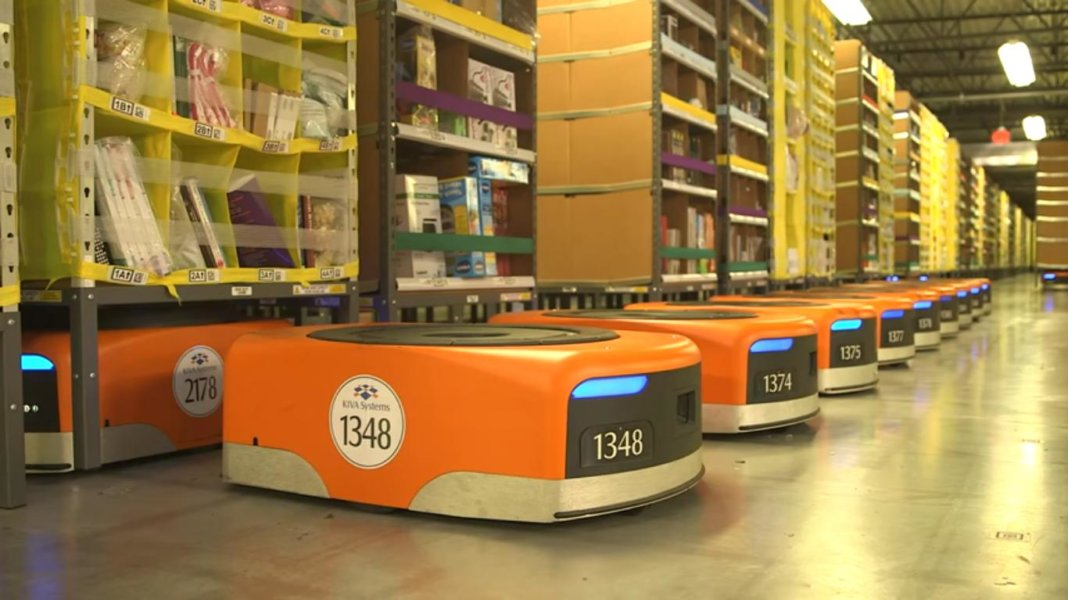
\includegraphics[width = 0.9\textwidth]{amazon}
        \end{center}
    \end{minipage}\hfill
    \begin{minipage}[c]{0.45\textwidth}
        \caption{Les robots Kiva d'\textsc{Amazon}}
        \label{figure:amazon}
    \end{minipage}
\end{figure}
\FloatBarrier

Des compagnies ont même poussé ce concept encore plus loin, créant des <<~entrepôts sans lumière~>>.
Comme \textsc{Siemens} qui possède des entrepôts capables de fonctionner dans le noir, de manière autonome, sans nécessiter le moindre être humain, et ce, pendant des semaines.
Ce genre d'entrepôts peut même permettre d'éliminer les besoins de climatisation ou de chauffage.

Dans des compagnies de taille moyenne, il est possible de mettre en place des systèmes capables d'anticiper les demandes de stocks à venir, et ainsi, pouvoir anticiper les achats nécessaires.

Pour réaliser de telles prédictions, les modèles les plus utilisés sont généralement des LSTM.
Un LSTM est un <<~long short-term memory~>>, c'est un réseau de neurones récurrents à mémoire court-terme et long terme.
C'est une version plus avancée d'un RNN qui convient mieux que ces derniers pour réaliser des prédictions.
Pour réaliser des prédictions solides, un tel modèle nécessite une quantité de données considérable, dans l'objectif de trouver des liens de cause à effet au sein de celles-ci.
Utiliser un tel système pour gérer les stocks au sein de \textsc{Disa} serait peu utile, car les données récoltées ne sont sûrement pas suffisantes.